\begin{figure}[h!]
\textbf{Tema d'Esame di Febbraio 2017}\\ \\
Sapendo che la resistenza $R8$ è attraversata da una corrente $i_8 = 0.20 A$, si calcoli la corrente che attraversa $R3$. Si considerino le seguenti resistenze $R8 = 10 \Omega, R1 = R2 = R3 = 5.0 \Omega , R4 = 12 \Omega , R5 = 15 \Omega $.
	\begin{center}
		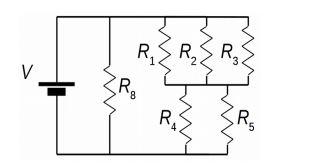
\includegraphics[scale=1.1]{ES5/FEB052017.jpg}
	\end{center}
	\begin{boxed}
		\null\hfill \textbf{Soluzione:} $I_3 = 0.08A$\\
		\textbf{Procedimento: } \\
		Semplificazione delle Resistenze:\\
		$R_{123}=\frac{1}{\frac{1}{R_1}+\frac{1}{R_2}+\frac{1}{R_3}}=\frac{1}{\frac{1}{5\Omega}+\frac{1}{5\Omega}+\frac{1}{5\Omega}}=1.67\Omega$\\ \\ 
		$R_{45}=\frac{R_4\cdot R_5}{R_4 + R_5}=\frac{12\Omega\cdot 15\Omega}{12\Omega + 15\Omega}=6.67\Omega$\\
		$R_{12345}=R_{123}+R_{45}=6.67\Omega+1.67\Omega=8.34\Omega$\\
		Ricordando che la tensione in parallelo non cambia, così come non cambia la corrente in serie:\\
		$V_{tot}=V_{12345}=V_8=R_8\cdot I_8=10\Omega\cdot 0.2A=2V$\\
		$I_{12345}=I_{123}=I_{45}=\frac{V}{R_{12345}}=\frac{2V}{8.34\Omega}=0.24A$\\
		$V_{123}=R_{123}\cdot I_{12345}=1.67\Omega\cdot 0.24A=0.40V$\\
		$I_3=\frac{V_{123}}{R_3}=\frac{0.40V}{5\Omega}=0.08A$
	\end{boxed}
\end{figure}

\begin{figure}[h!]
\textbf{Tema d'Esame di Giugno 2017}\\ \\
 Si determini il valore della resistenza $R_x$ del circuito mostrato nella figura sotto a sinistra. La differenza di potenziale fornita dalla batteria è $3 V$, la corrente i3 che scorre nella resistenza $R3$ è pari a $0.1 A$ ed i valori delle altre resistenze nel circuito
sono $R1 = R2 = 5 \Omega ,R3 = R4 = 10 \Omega$.
\begin{center}
		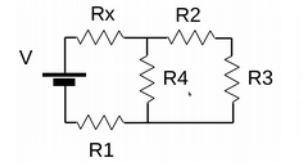
\includegraphics[scale=1.1]{ES5/GIU052017.jpg}
	\end{center}
\end{figure}

\begin{figure}[h!]
\textbf{Tema d'Esame di Settembre 2017}\\ \\
Trovare le correnti $i_1, i_2 , i_3$ nei tre rami del circuito qui sotto.
$R1 = 4.0 \Omega, R2 = 6.0 \Omega, R3 = 3.0 \Omega$ ed $ E 1 = 1.5 V,  E 2 = 3.0 V$.
\begin{center}
		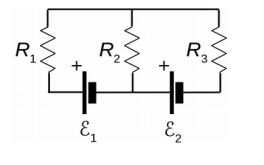
\includegraphics[scale=1.1]{ES5/SET052017.jpg}
	\end{center}
\end{figure}